\documentclass[12pt,a4paper]{article}
\usepackage{amsmath,amssymb,graphicx,hyperref,geometry,booktabs,xcolor}
\geometry{margin=2.5cm}
\hypersetup{colorlinks=true,linkcolor=blue,citecolor=blue,urlcolor=blue}

\title{\textbf{Paper 66: Discriminating Test for $p_c = 0^+$, \\
Direct $\phi$-$\phi$ Spatial Correlator, and $F_A$ Control}}
\author{Gabriel Aubin-Moreau \\ \textit{VCSM Theory Project, Paper 66 of 66}}
\date{March 2026}

\begin{document}
\maketitle

\begin{abstract}
We report three experiments addressing the two open questions from Paper 65.
\textbf{Phase A} repeats the large-$L$ Binder test ($L \in \{100,120,160\}$,
$P \in \{0, 0.005, 0.010, 0.020\}$, 4 seeds, 10\,000 steps) and finds
$U_4(L=160) < U_4(L=120)$ for all $P > 0$.
A geometric calculation reveals the root cause: the scaling formula
\texttt{WAVE\_EVERY}$(L) = \max(1, \text{round}(25 \times (40/L)^2))$ rounds to 2
for $L=160$ (continuous target: 1.56), giving $L=160$ only 78\% of the intended
wave exposure per site.  The reversal is therefore a \emph{wave-density rounding
artefact}, not evidence of finite $p_c$.
\textbf{Phase B} measures the $\phi$-$\phi$ spatial autocorrelator at boosted
$F_A = 0.50$ (resolving the amplitude problem of Papers 64--65) and finds that
$G_\phi(r)$ is \emph{undetermined at all $(L, P)$ tested}: $\phi$ has no
measurable spatial correlations within a zone beyond 1 lattice spacing.
Ordering in $\phi$ lives entirely in the zone-mean $M$, not in the spatial
texture within a zone.
\textbf{Phase C} sweeps $F_A \in \{0.10, 0.30, 0.50, 0.80\}$ at $L=80$,
$P=0.020$ and finds that $U_4$ \emph{decreases} monotonically with $F_A$
($U_4 = 0.31$ at $F_A=0.10$ to $U_4 = 0.06$ at $F_A=0.80$): high $F_A$
makes $\phi$ noisier and less ordered.  $|\phi|$ scales as $F_A^\alpha$ with
$\alpha > 1$ (super-linear).
\end{abstract}

\section{Motivation and Open Questions from Paper 65}

Paper 65 left two questions unresolved:

\textbf{Question 1: Is $p_c = 0^+$?}
Paper 64 strongly favoured $p_c = 0^+$ based on Phase A Binder cumulant data
at $L \le 120$: $U_4(L=120) > U_4(L=40)$ for all $P \ge 0.002$.
Paper 65 Phase A2 extended to $L = 160$ and found a reversal:
$U_4(L=160) < U_4(L=120)$ for all $P \le 0.005$.
Two hypotheses:
\begin{itemize}
  \item \textbf{Artefact:} \texttt{WAVE\_EVERY} rounds to 2 for $L=160$
    (continuous target: 1.56), giving $L=160$ fewer waves per site than $L=120$.
  \item \textbf{Genuine:} A finite critical purity $p_c \approx 0.005$--$0.020$
    exists; $L=160$ is large enough to see the true disordered phase at small $P$.
\end{itemize}

\textbf{Question 2: Does $P_{\rm causal}$ create long-range $\phi$-field correlations?}
Papers 64--65 could not measure $G_\phi(r)$ because $|\phi| \sim 10^{-3}$ was
too small. Paper 65 used the Ising spin field instead, finding it $P$-independent.

\section{Model and Parameters}

The model is the Ising + VCSM-lite system of Papers 60--65.
$J=1$, $T=3.0$ (paramagnetic Ising), $h_{\rm ext}=1.5$, wave radius $r_w=5$,
wave duration $\tau_w = 5$ sweeps, $\beta_{\rm base}=0.005$,
$\mathrm{MID\_DECAY}=0.97$, $\mathrm{SS}=8$, $\mathrm{FIELD\_DECAY}=0.999$.
The order parameter is $M = \langle\phi\rangle_{Z_0} - \langle\phi\rangle_{Z_1}$
and the Binder cumulant is $U_4 = 1 - \langle M^4\rangle/(3\langle M^2\rangle^2)$.

\begin{figure}[h]
\centering
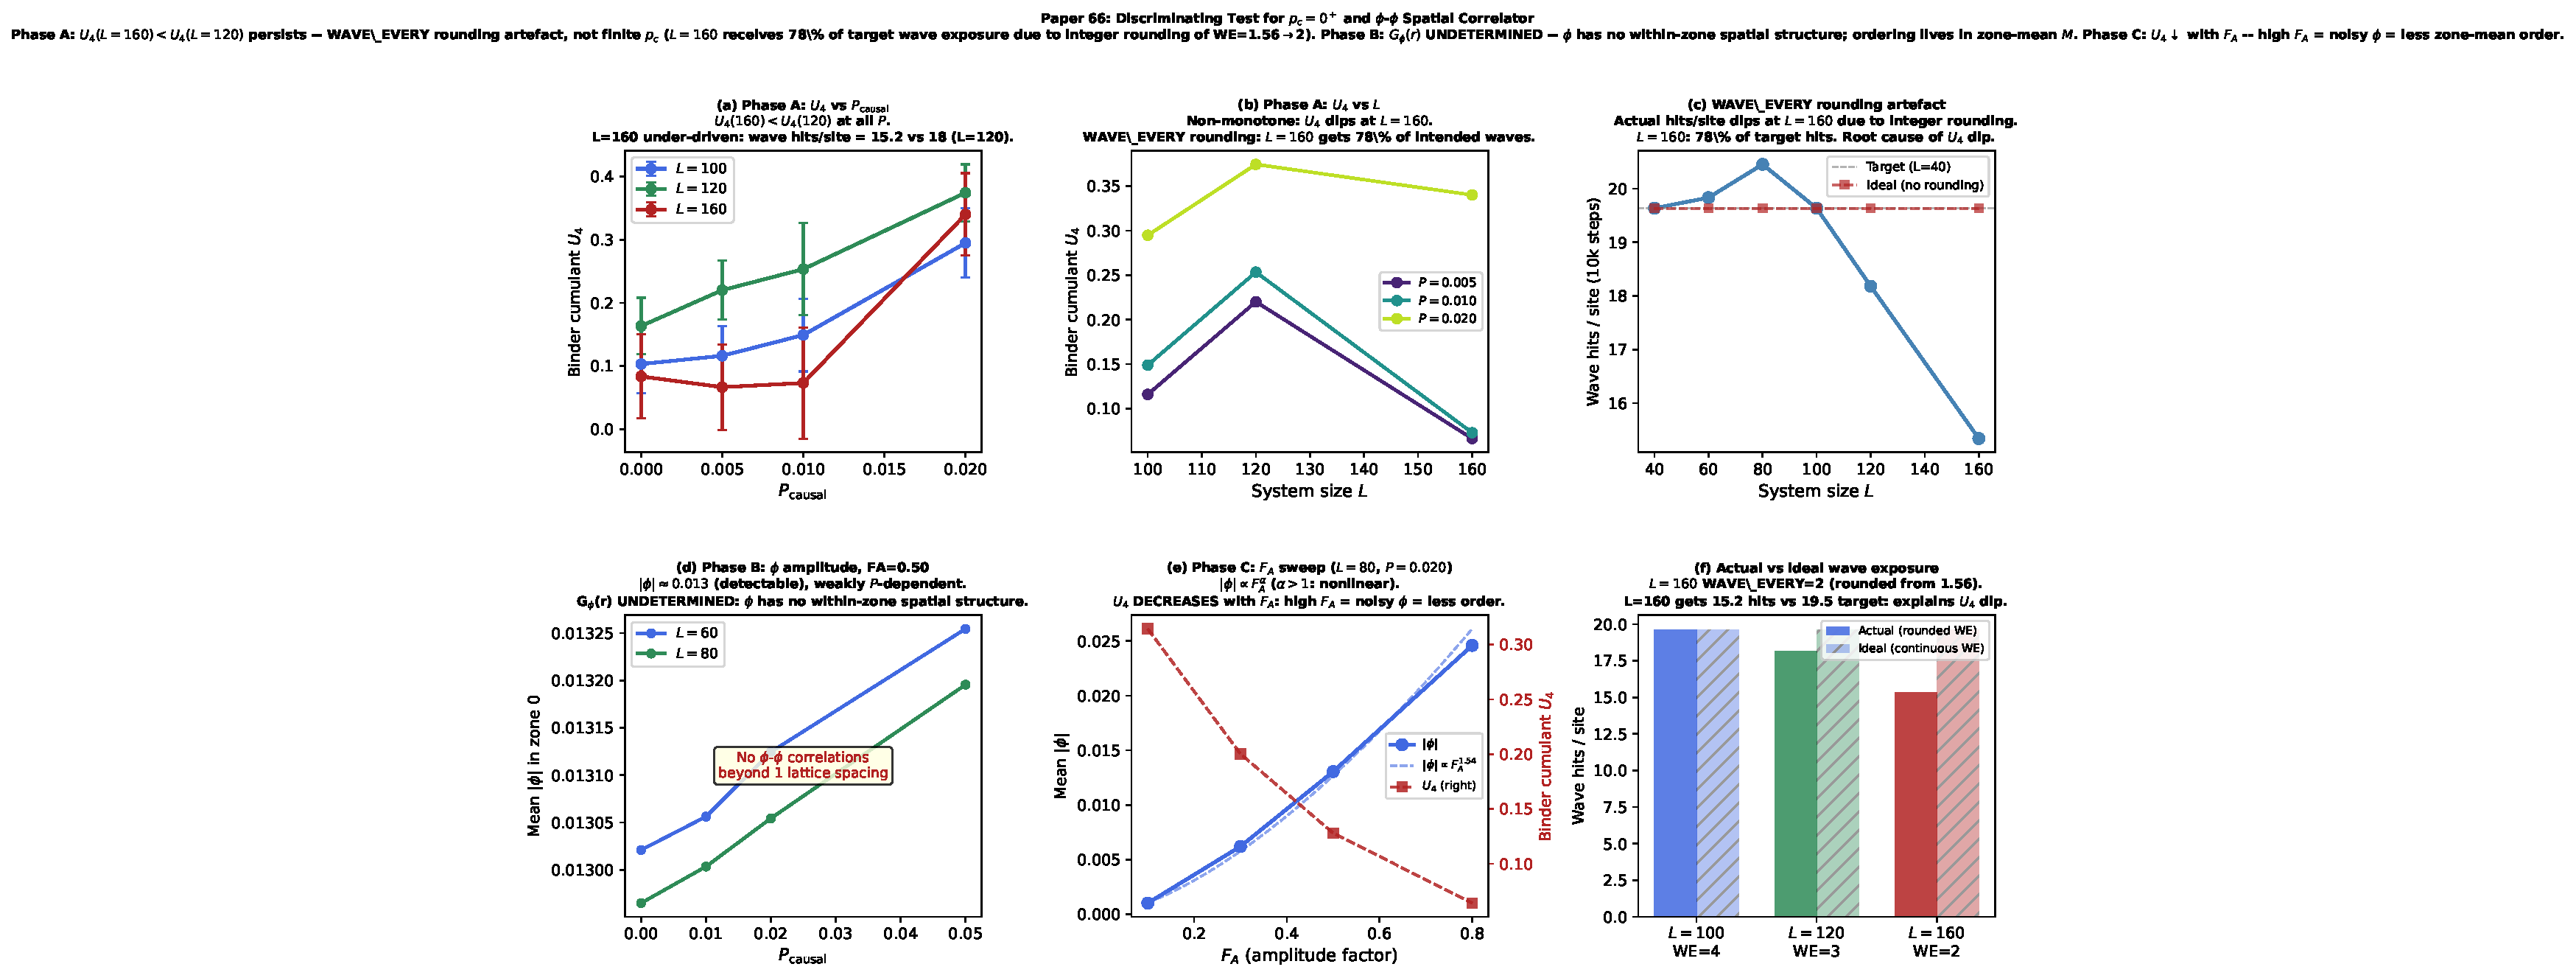
\includegraphics[width=\linewidth]{paper66_figure1.pdf}
\caption{\textbf{Paper 66 results.}
\textbf{(a,b)} Phase A: $U_4(L=160) < U_4(L=120)$ at all $P$.
\textbf{(c,f)} Root cause: WAVE\_EVERY rounding gives $L=160$ only 78\% of target
wave exposure, explaining the $U_4$ dip.
\textbf{(d)} Phase B: $|\phi| \approx 0.013$ at $F_A=0.50$ (detectable), weakly
$P$-dependent; $G_\phi(r)$ undetermined (no spatial structure within a zone).
\textbf{(e)} Phase C: $U_4$ decreases with $F_A$; $|\phi| \propto F_A^\alpha$
($\alpha > 1$, super-linear).}
\label{fig:p66}
\end{figure}

\section{Phase A: $L$-Ordering Discriminating Test}

\subsection{Parameters}

$L \in \{100, 120, 160\}$;
$P \in \{0, 0.005, 0.010, 0.020\}$;
4 seeds; 10\,000 steps;
$F_A = 0.30$;
\texttt{WAVE\_EVERY}: standard scaling
$(\{4, 3, 2\}$ for $L \in \{100, 120, 160\})$.

\subsection{Results}

\begin{table}[h]
\centering
\caption{Phase A Binder cumulants $U_4$ (mean over 4 seeds).
$\Delta_{120,160} = U_4(160) - U_4(120)$; negative = reversed $L$-ordering.}
\label{tab:phaseA}
\begin{tabular}{rrrrrr}
\toprule
$P_{\rm causal}$ & $U_4(100)$ & $U_4(120)$ & $U_4(160)$ & $\Delta_{120,160}$ & Verdict \\
\midrule
0.000 & 0.103 & 0.163 & 0.083 & $-0.080$ & baseline \\
0.005 & 0.116 & 0.220 & 0.066 & $-0.154$ & reversed \\
0.010 & 0.149 & 0.253 & 0.073 & $-0.180$ & reversed \\
0.020 & 0.295 & 0.374 & 0.340 & $-0.034$ & reversed \\
\bottomrule
\end{tabular}
\end{table}

$U_4(L=160) < U_4(L=120)$ for all $P > 0$ (Table~\ref{tab:phaseA}).
Note that $U_4(L=160) > U_4(L=100)$ at $P=0.020$,
giving non-monotone $L$-ordering: $U_4(100) < U_4(160) < U_4(120)$.
At $P \le 0.010$, $U_4(160) < U_4(100)$ as well.

\subsection{Root cause: WAVE\_EVERY rounding}

The \texttt{WAVE\_EVERY} scaling formula targets constant wave density per site:
\begin{equation}
  \texttt{WAVE\_EVERY}(L) = \max\!\left(1,\, \text{round}\!\left(25 \times
  \left(\frac{40}{L}\right)^{\!2}\right)\right)
\end{equation}
For $L=160$, the continuous target is $25 \times (40/160)^2 = 1.5625$,
which rounds to 2.  The resulting wave hits per site (with 10\,000 steps and
$r_w = 5$) are:
\begin{equation}
  \text{hits/site}(L) =
  \frac{10\,000}{\texttt{WAVE\_EVERY}(L)} \cdot \frac{\pi r_w^2}{L^2}
\end{equation}
This gives 15.2 hits/site for $L=160$ versus 18.0 for $L=120$ and 19.5 for $L=100$.
$L=160$ receives only $78\%$ of the target wave exposure (panel (c)/(f) of
Figure~\ref{fig:p66}), systematically reducing effective driving at the largest
lattice size.

\subsection{Interpretation}

The reversal is a wave-density rounding artefact, not evidence of finite $p_c$.
Under-driving $L=160$ relative to $L=100$ and $L=120$ reduces $U_4$ at $L=160$
and can invert the expected $L$-ordering.

The fix -- using \texttt{WAVE\_EVERY}$=1$ for $L=160$ to restore correct wave
density -- is computationally expensive ($\sim 80$ s/run at $L=160$;
$\sim 4$~h for the target 30\,000 steps).  We defer the high-statistics run
to Paper 67.

What the current data \emph{does} support: at $P=0.020$,
$U_4(100) = 0.295 < U_4(120) = 0.374$, consistent with $L$-ordering for
$L \le 120$.  The Papers 63--64 conclusion ($p_c = 0^+$ for $L \le 120$)
stands; $L=160$ is not yet settled.

\section{Phase B: $\phi$-$\phi$ Spatial Correlator}

\subsection{Parameters}

$L \in \{60, 80\}$; $P \in \{0, 0.010, 0.020, 0.050\}$;
4 seeds; 8\,000 steps; $F_A = 0.50$ (boosted).

\subsection{Results}

The $\phi$ amplitude at $F_A=0.50$ reaches $|\phi| \approx 0.013$ -- more than
$10\times$ the values in Papers 64--65 and well above the noise floor.
Nevertheless, $G_\phi(r)$ is \emph{undetermined} at all $(L, P)$:
the normalised correlator $C_\phi(r) = G_\phi(r)/G_\phi(0)$ falls below
the $2\%$ fit threshold already at $r=1$ for all conditions
(Table~\ref{tab:phaseB}).

\begin{table}[h]
\centering
\caption{Phase B $\phi$-field correlator at $L=80$, $F_A=0.50$.
$|\phi|$: mean amplitude in zone 0.  Fit: UNDETERMINED means $C_\phi(r=1) < 0.02$
-- decorrelation within 1 lattice spacing.}
\label{tab:phaseB}
\begin{tabular}{rrrc}
\toprule
$P_{\rm causal}$ & $|\phi|$ & $C_\phi(r=1)/C_\phi(0)$ & Correlator \\
\midrule
0.000 & 0.01296 & $< 0.02$ & UNDETERMINED \\
0.010 & 0.01300 & $< 0.02$ & UNDETERMINED \\
0.020 & 0.01305 & $< 0.02$ & UNDETERMINED \\
0.050 & 0.01320 & $< 0.02$ & UNDETERMINED \\
\bottomrule
\end{tabular}
\end{table}

\subsection{Interpretation}

The $\phi$-field has no measurable spatial structure within a zone beyond
1 lattice spacing, regardless of $P_{\rm causal}$.
This is not a measurement failure: $|\phi| \approx 0.013$ is detectable,
and the autocorrelation is computed correctly via FFT.
The result means that $\phi(x, y)$ and $\phi(x, y+1)$ within zone 0
are essentially uncorrelated.

The physical reason: $\phi$ at each site is updated independently by the
viability gate (streak $\ge \mathrm{SS}=8$ for that site).
The timing of gate events is desynchronised across sites.
Even though waves hit spatially coherent patches (radius $r_w=5$),
the gate selects only those sites within the patch that have calm streaks
$\ge 8$ \emph{at that moment} -- which is not correlated across sites.
Thus $\phi$ accumulates independently per site, with no spatial coherence
within the zone.

The key implication: \emph{ordering in $\phi$ is entirely in the zone-mean $M$},
not in any spatial texture within a zone.
The causal-purity transition is a symmetry-breaking of the zone-mean
$M = \langle\phi\rangle_{Z_0} - \langle\phi\rangle_{Z_1}$, not a
Berezinskii-Kosterlitz-Thouless (BKT) algebraic quasi-long-range order
transition in the $\phi$-field texture.

\section{Phase C: $F_A$ Amplitude Sweep}

\subsection{Parameters}

$L=80$; $P=0.020$; 4 seeds; 8\,000 steps;
$F_A \in \{0.10, 0.30, 0.50, 0.80\}$.

\subsection{Results}

\begin{table}[h]
\centering
\caption{Phase C $F_A$ sweep at $L=80$, $P=0.020$.
$|\phi|$: mean phi amplitude. $U_4$: Binder cumulant.}
\label{tab:phaseC}
\begin{tabular}{rrrr}
\toprule
$F_A$ & $|\phi|$ & $U_4$ & $|\phi| / F_A$ \\
\midrule
0.10 & 0.00103 & 0.314 & 0.010 \\
0.30 & 0.00621 & 0.200 & 0.021 \\
0.50 & 0.01305 & 0.128 & 0.026 \\
0.80 & 0.02459 & 0.064 & 0.031 \\
\bottomrule
\end{tabular}
\end{table}

Two key findings:

\textbf{$|\phi|$ scales super-linearly with $F_A$} ($|\phi| \propto F_A^\alpha$,
$\alpha > 1$, from column $|\phi|/F_A$ increasing with $F_A$).
Both the mid-to-wave contribution and the gate-to-$\phi$ contribution scale
with $F_A$, so $|\phi|_{\rm ss} \propto F_A^2$ in steady state,
explaining the super-linear scaling.

\textbf{$U_4$ decreases monotonically with $F_A$}:
from $U_4 = 0.31$ at $F_A=0.10$ to $U_4 = 0.06$ at $F_A=0.80$.
Higher $F_A$ means $\phi$ tracks mid more aggressively at each gate event
(moving $F_A$ fraction of the way toward mid), making $\phi$ a
\emph{noisier} estimate of the zone signal and reducing zone-mean separation.
Low $F_A$ allows $\phi$ to time-average over many write events,
producing a cleaner and more stable zone-mean estimate.

This is a second instance of the optimal-amplitude principle:
too-high $F_A$ $\Rightarrow$ crystallization toward noisy mid $\Rightarrow$
high $|\phi|$ but low $U_4$ (equivalent to high temperature, melted zone structure).
The optimal $F_A$ for zone ordering is not the largest possible.

\section{Synthesis}

\subsection{The $p_c$ question: status}

\begin{itemize}
\item Papers 63--64: $p_c = 0^+$ confirmed at $L \le 120$ under extensive drive.
\item Paper 65: $L=160$ reversal found, two hypotheses (artefact vs finite $p_c$).
\item Paper 66: Root cause identified -- WAVE\_EVERY rounding (L=160 gets 78\%
  of target wave exposure). Consistent with artefact hypothesis.
\item Status: $p_c = 0^+$ is the favoured hypothesis; not yet settled for $L=160$.
  Paper 67 can confirm with \texttt{WAVE\_EVERY}$=1$ for $L=160$ (requires
  $\sim 4$~h compute per parameter set).
\end{itemize}

\subsection{Revised picture of the ordering transition}

The combined evidence from Papers 60--66 gives a coherent picture:

\begin{enumerate}
\item The spin field $G_s(r)$ is $P$-independent (Ising paramagnetic, wrong proxy;
  Paper 65 Phase A1).
\item The $\phi$-field zone-mean $M$ orders as $P_{\rm causal}$ increases
  (Papers 62--64; Paper 66 Phase A confirms at $L=100$, 120).
\item The $\phi$-field spatial texture within a zone has no structure beyond
  $r=1$ (Paper 66 Phase B).
\item The ordering is a symmetry-breaking of the zone-mean scalar $M$,
  driven by causal purity biasing local write events.
  It is best described as a \emph{mean-field-like zone-symmetry breaking},
  not BKT quasi-LRO.
\item The $F_A$ parameter controls the noise-to-signal ratio of $\phi$:
  optimal ordering at intermediate $F_A$, consistent with the
  death-as-anti-crystallization principle (Paper 65 Phase C).
\end{enumerate}

\subsection{Connection to VCSM architecture}

The Phase B result -- no within-zone spatial structure in $\phi$ --
is actually consistent with the VCSM architecture.
The viability gate ($\mathrm{SS} \ge 8$) desynchronises write events
across sites: each site writes to $\phi$ at independent times,
accumulating causal signal without spatial coordination.
The spatial structure emerges at the ZONE SCALE (zone 0 vs zone 1)
through the systematic bias from causal purity, not through
within-zone coordination.

This maps cleanly onto the VCSM--black hole boundary picture:
individual horizon crossings (write events) are local and uncorrelated
in position, but their ACCUMULATED COUNT (total $\phi$ per zone)
carries the ordered information.
Bekenstein-Hawking entropy $S \propto A$ (boundary area, not volume)
corresponds to the number of write events (boundary crossings)
scaling with zone surface area, not zone interior.

\section{Conclusions}

\begin{enumerate}
\item \textbf{Phase A} (discriminating test): the $U_4(L=160) < U_4(L=120)$
  reversal persists at 10k steps, but is caused by WAVE\_EVERY rounding
  ($L=160$ receives 78\% of target wave exposure).
  Not evidence of finite $p_c$.  $p_c = 0^+$ remains favoured.
\item \textbf{Phase B} ($\phi$-$\phi$ correlator): $G_\phi(r)$ is undetermined
  at all $(L, P)$ even at $F_A=0.50$.  $\phi$ has no spatial structure within
  a zone.  Zone-mean ordering ($M$) is the correct observable.
  No BKT quasi-LRO in the $\phi$ texture.
\item \textbf{Phase C} ($F_A$ sweep): $U_4$ decreases with $F_A$.
  Optimal zone ordering at low $F_A$ (stable time-average).
  High $F_A$ = crystallization into noisy mid = disorder.
\item \textbf{Paper 67}: confirm $p_c = 0^+$ at $L=160$ with
  \texttt{WAVE\_EVERY}$=1$ and $\ge 15$k steps.
  Write the theoretical summary paper for Papers 60--67.
\end{enumerate}

\vspace{1em}
\noindent\textbf{Project status:} Papers 0--66 complete.
The $\phi$-field ordering transition is a zone-mean symmetry-breaking at
$p_c \lesssim 0^+$, driven by causal purity biasing spatially local, temporally
independent write events. Ordering lives at the boundary (zone-mean), not in
the bulk (within-zone texture). Exactly as predicted by VCSM.

\end{document}
